%%%%%%%%%%%%%%%%%%%%%%%%%%%TBP on h-BN/Cu(111)
\label{section:TBP-on-hBN}
\begin{figure}[] \centering
	\subfigure[\textit{h}-BN grown on Cu(111).]{
		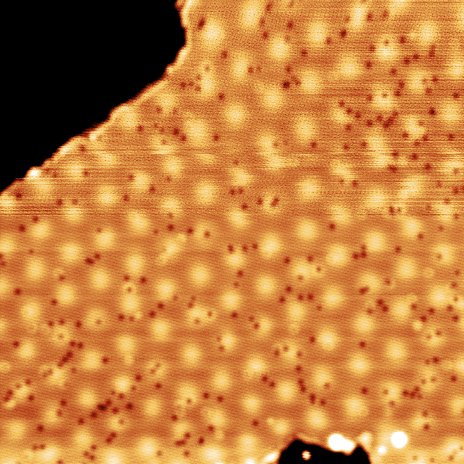
\includegraphics[width=0.3\textwidth]{./images/F151130-135150-40nm.png}
		\label{fig:h-BN-Cu111}
	}
	\subfigure[TBP after adsorption on \textit{h}-BN/Cu(111)]{
		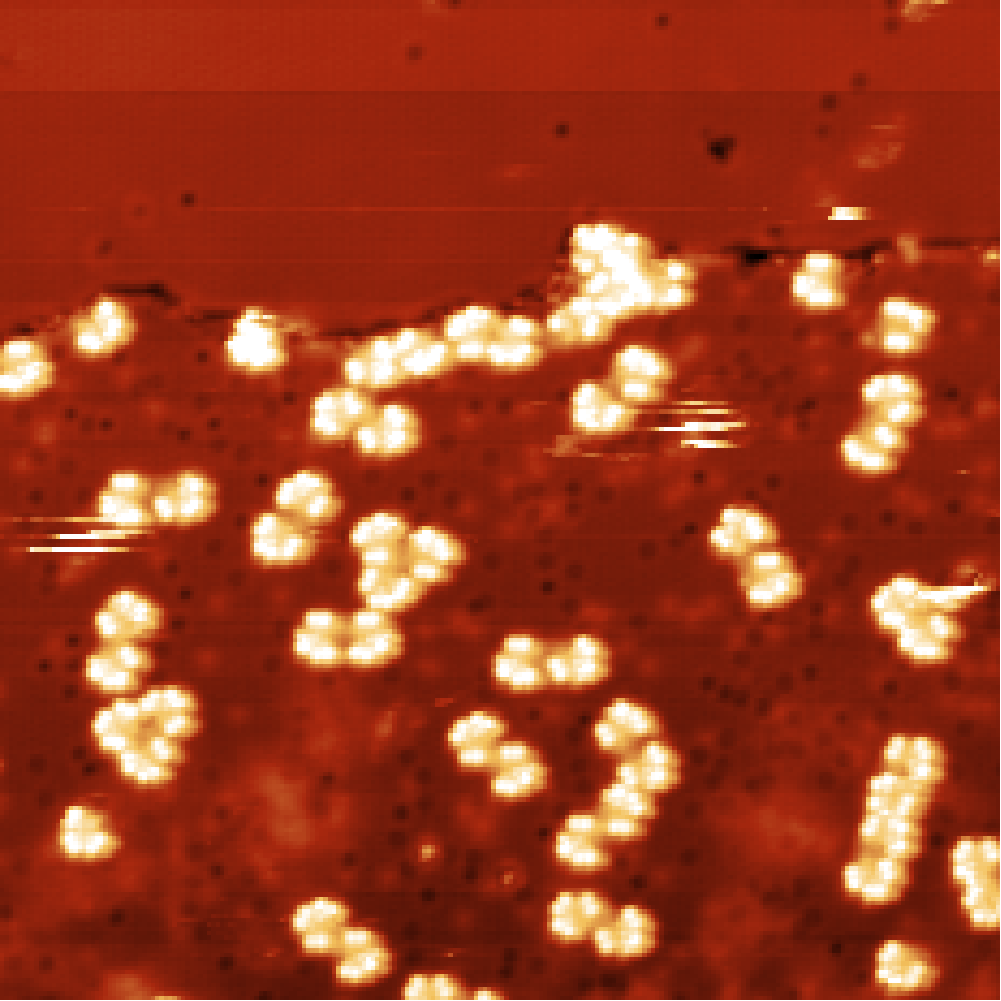
\includegraphics[width=0.3\textwidth]{./images/F160617-110201-40nm.png}
		\label{fig:single-TBP-hBN-cu111}
	}
	\subfigure[TBP after adsorption on \textit{h}-BN/Cu foil.]{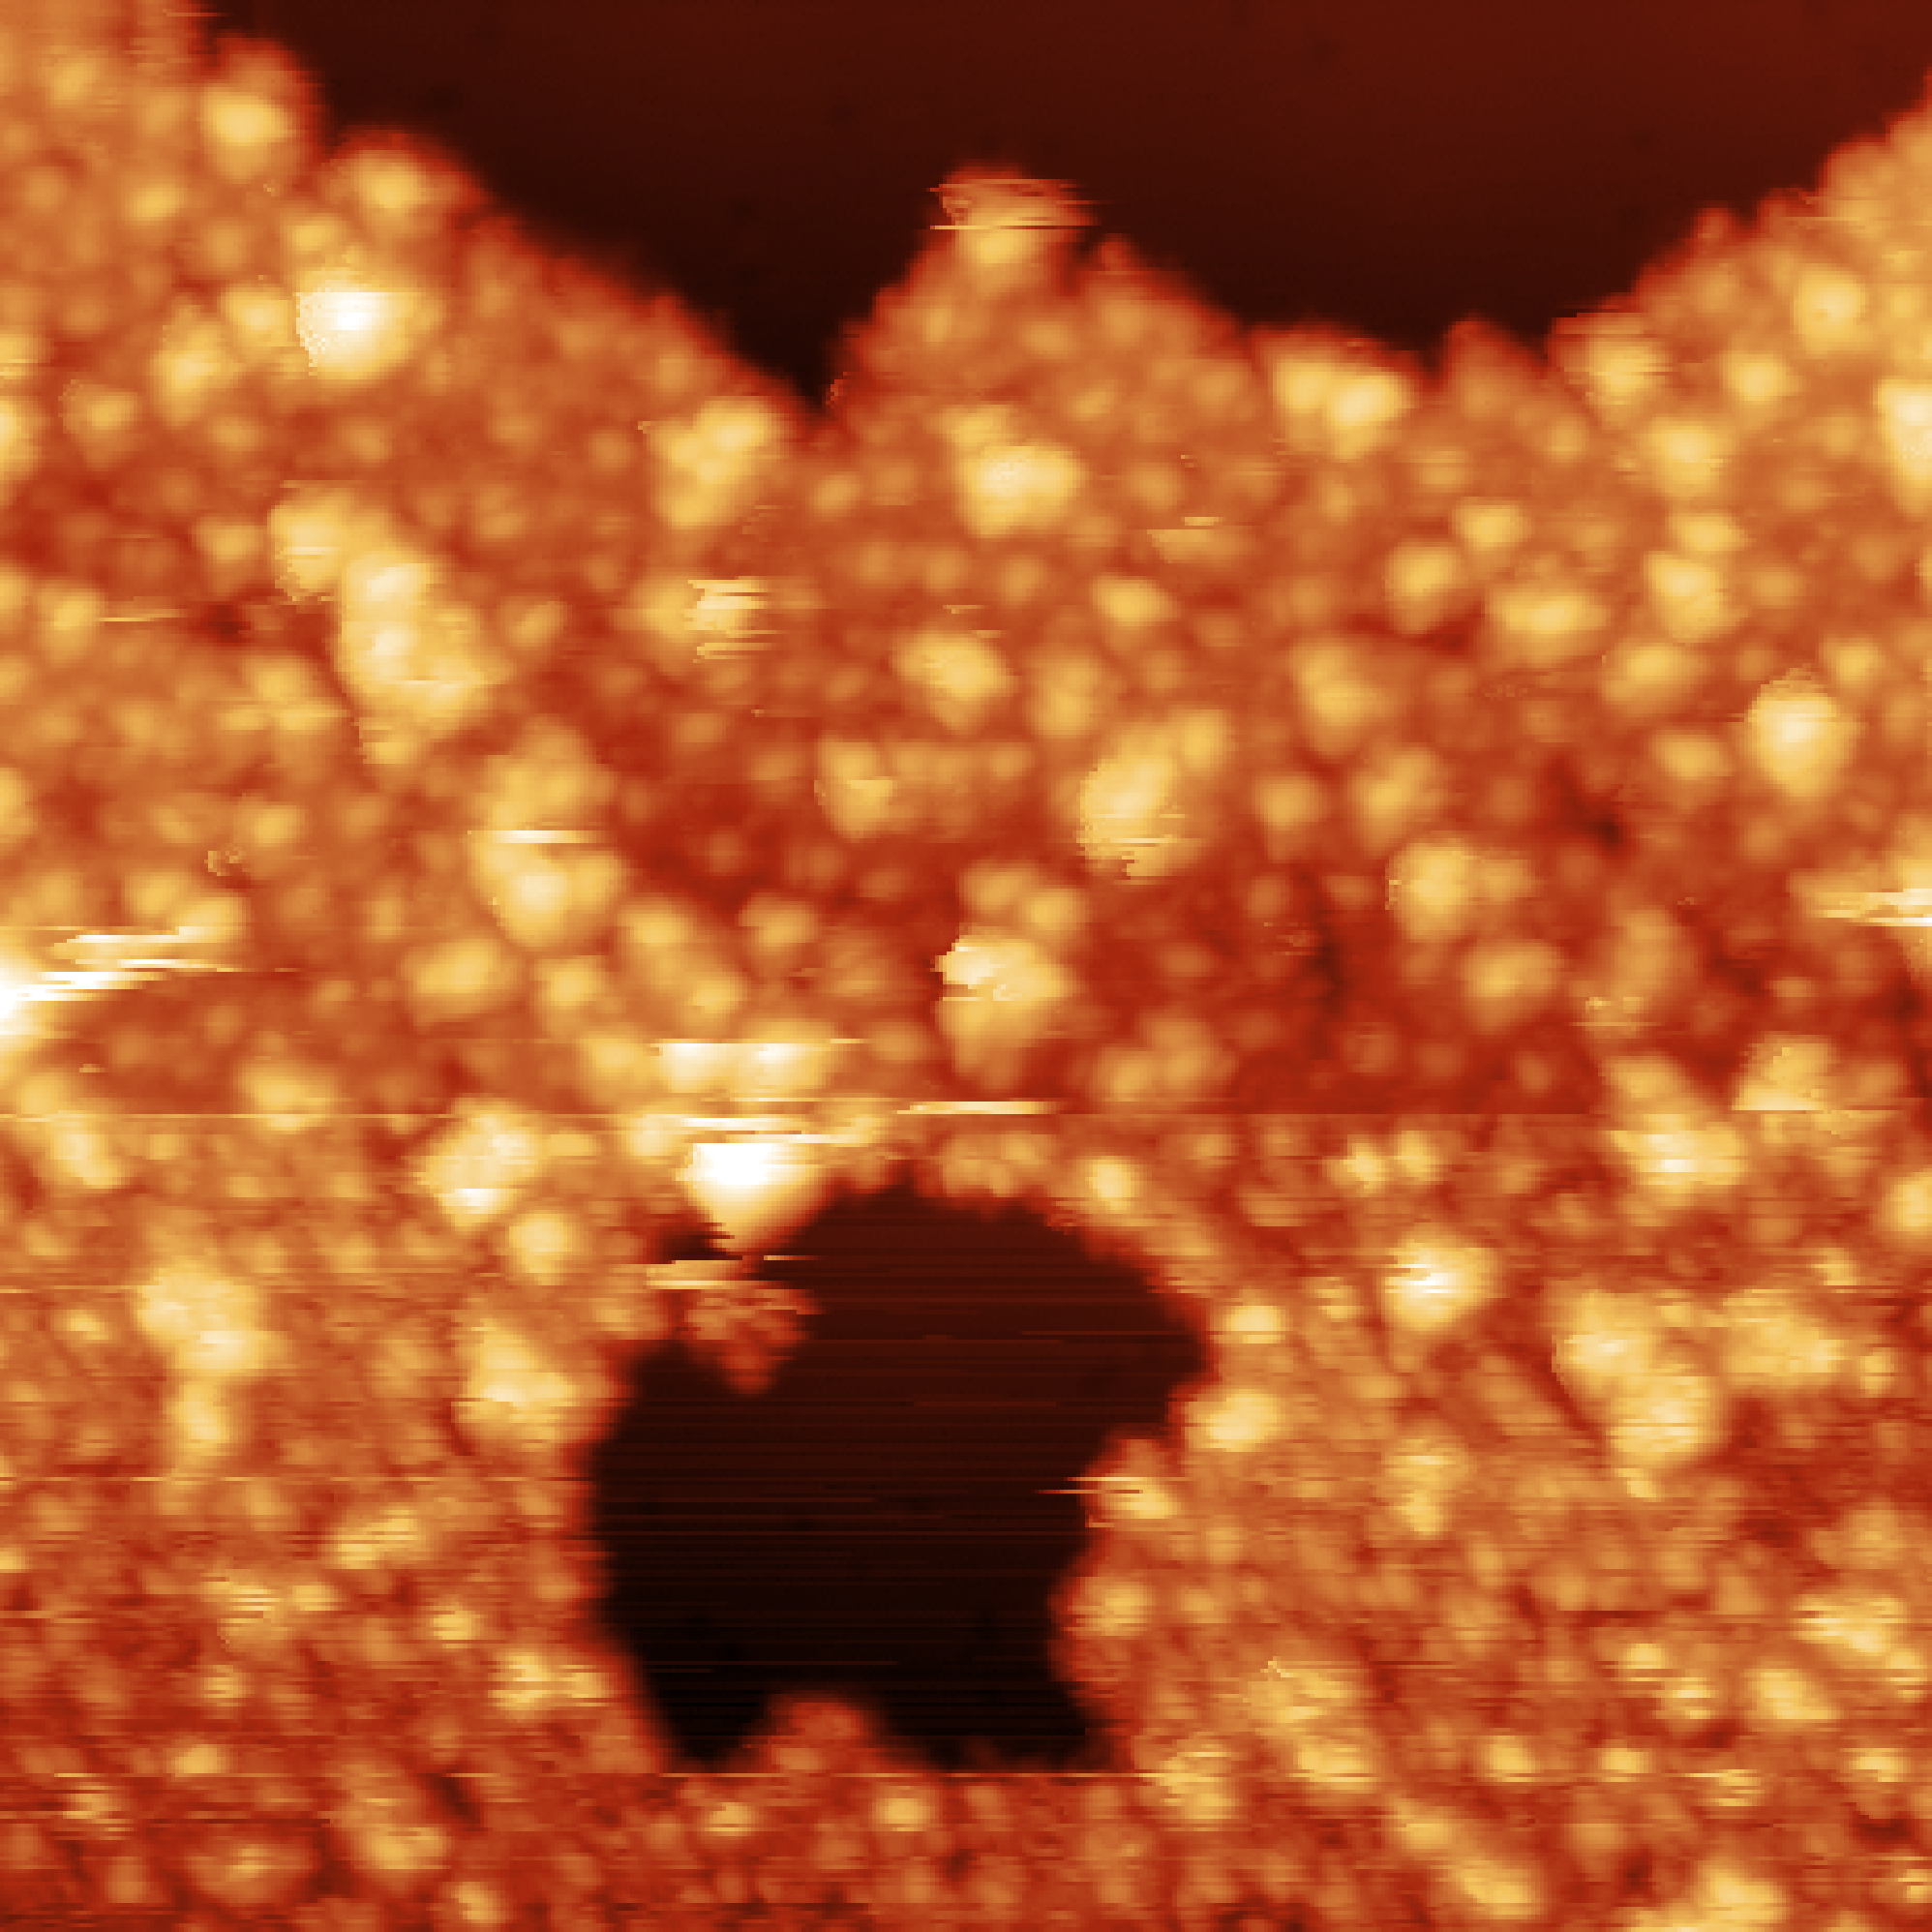
\includegraphics[width=0.3\textwidth]{./images/F151123-110602-40nm.png}
		\label{fig:single-TBP-hBN-cu-foil}
	}
	\caption{STM topographs of \textit{h}-BN grown on copper with subsequent molecular adsorption. \subref{fig:h-BN-Cu111} shows a \textit{h}-BN layer grown on Cu(111) by CVD. \subref{fig:single-TBP-hBN-cu111} shows the sample after evaporating TBP molecules at RT. \subref{fig:single-TBP-hBN-cu-foil} shows empty \textit{h}-BN islands grown on the polycrystalline copper foil and molecules on a copper terrace. 
		Scan parameters: \subref{fig:h-BN-Cu111} $U_b=\SI{2.273}{\volt}, I_t=\SI{0.048}{\nano \ampere}$, color scale \SIrange{0}{100}{\pico \meter}. \subref{fig:single-TBP-hBN-cu111} $U_b=\SI{1.074}{\volt}, I_t=\SI{0.033}{\nano \ampere}$, color scale \SIrange{0}{300}{\pico \meter}. \subref{fig:single-TBP-hBN-cu-foil} $U_b=\SI{2.585}{\volt}, I_t=\SI{0.032}{\nano \ampere}$, color scale \SIrange{0}{1500}{\pico \meter}.  All images are \SI{40}{\nano \meter} wide.}
	\label{TBP-on-hBN}
\end{figure}

\paragraph{\textit{h}-BN grown on Cu(111)}
\textcolor{red}{\textbf{
Further experiments have can done to investigate the behavior of TBP on \textit{h}-BN. When adsorbed on \textit{h}-BN/Cu(111), molecules show a high mobility that makes the molecules move away from the \textit{h}-BN islands. Some molecules could be resolved at defects or close to the perimeter of the \textit{h}-BN islands. This is in line with other observations for adsorbates ((CITATION)). Adsorption temperatures as low as \SI{-170}{\celsius} have been used to lower the molecules' energy pool, but diffusion to free metal areas occurs and no molecules remain on the \textit{h}-BN surface.
}}

%single-TPB-on-h-bn-cu-foil
\paragraph{\textit{h}-BN grown on Cu-foil}
\textcolor{red}{\textbf{
Molecules adsorb on the BN surface and STM imaging is hard due to molecules that can be moved on the rather 'slippy' surface of the insulating BN. Nevertheless some agglomerations of the molecules leave free BN spots where no molecules are. As the preparation of the BN should result in a closed BN layer on top of the Cu-foil no movement of molecules to free Cu areas should be observed, making these free regions BN regions.
Why the molecules are not distributed homogenously on the BN remains topic to speculation.
Spectroscopy has been tried intensively but without reproduceable results.
Unlike the adsorption on Ag(100) and Cu(111) no formation of di- and quatermers has been observed.
% See experiments in June '16
}}